%\documentstyle[epsf,twocolumn]{jarticle}       %LaTeX2.09仕様
%\documentclass[twocolumn]{jarticle}     %pLaTeX2e仕様
\documentclass{jarticle}     %pLaTeX2e仕様

%一枚組だったら[twocolumn]関係のとこ消す

\setlength{\topmargin}{-45pt}
%\setlength{\oddsidemargin}{0cm} 
\setlength{\oddsidemargin}{-7.5mm}
%\setlength{\evensidemargin}{0cm} 
\setlength{\textheight}{24.1cm}
%setlength{\textheight}{25cm} 
\setlength{\textwidth}{17.4cm}
%\setlength{\textwidth}{172mm} 
\setlength{\columnsep}{11mm}

\kanjiskip=.07zw plus.5pt minus.5pt

\usepackage{graphicx}
\usepackage[dvipdfmx]{color}
\usepackage{subcaption}
\usepackage{enumerate}
\usepackage{comment}
\usepackage{url}
\usepackage{multirow}
\usepackage{diagbox}
\usepackage{amsmath,amssymb}
\usepackage{mathtools}
\usepackage{wrapfig}
\usepackage{graphicx}


\begin{document}
  \noindent
  \onecolumn
  \hspace{1em}

  \today
  \hfill
  \ \ B3 西村昭賢 

  \vspace{2mm}
  \hrule
  \begin{center}
  {\Large \bf 進捗報告}
  \end{center}
  \hrule
  \vspace{3mm}


\section{今週やったこと}

\begin{quote}
  \begin{itemize}
   \item Docker の環境構築
   \item 自作カードゲーム環境の改良と実験
  \end{itemize}
 \end{quote}


\section{Docker の環境構築}
先週まで上手く行かなかったが,先週火曜の B3 実験の時間
に先輩方にご教授頂きいろいろ試行錯誤した結果サーバー使って実験できるようになった.
坂川さん岡本さんありがとうございます.


\section{カードゲーム環境の改良と実験}
先週までは,予め決まった盤面状況の中でデッキから手札へのドロー,手札から盤面のプレイなどを考えずに自プレイヤーの行動→敵プレイヤーの行動を1エピソードとする学習しか実現できなかった.
今週は先週検討した予め盤面と手札の最大枚数を決定し行動空間と状態空間を予め定めておく方法を軸に実装をし\cite{実装},ゲーム開始から終了までを1エピソードとした実験を回せるように環境を改良した.また,改良した環境で実験した.

\subsection{カードゲームのルール}
先週森先生に頂いたアドバイスを踏まえてプレイヤーの体力やカードのコストは実装せずに簡単なルールのカードゲームを作成した.

\begin{quote}
  \begin{itemize}
   \item プレイヤー
   \par
   プレイヤーは最大 9 枚の手札,最大 5 枚まで盤面にカードを持つことができる.枚数制限を超えた場合, 新たに加えようとしたカードは破壊される.
   ゲーム開始時にデッキから3枚ドローする.
   その後はターンが回ってくると自動でデッキから1枚ドローする.
   \item カード
   \par
   カードは攻撃力と HP を持つ.相手のカードに攻撃することができ,攻撃した際には攻撃対象のカードの攻撃力分ダメージを受ける.
   \item デッキ
   \par
   15枚のカードからなる.ゲーム開始時にシャッフルされる.
   \item 終了条件
   \par
   お互いのプレイヤーのデッキ,手札の両方からカードが無くなったらゲーム終了.
   \item 勝利条件
   \par
   盤面のカード枚数が多いプレイヤーの勝利.カードの枚数が同じだった場合には盤面のカードの攻撃力と HP の総和を計算し, (先攻プレイヤーの総和) $\geqq$ (後攻プレイヤーの総和)ならば先攻プレイヤーの勝利,そうでなければ後攻プレイヤーの勝利.
  \end{itemize}
 \end{quote}

\subsection{行動空間の次元}
以前から述べているが, OpenAI Gym に自作環境を定義する際は行動空間の次元,状態空間,報酬を定義する必要がある.

\begin{figure}[htbp]
  \centering
  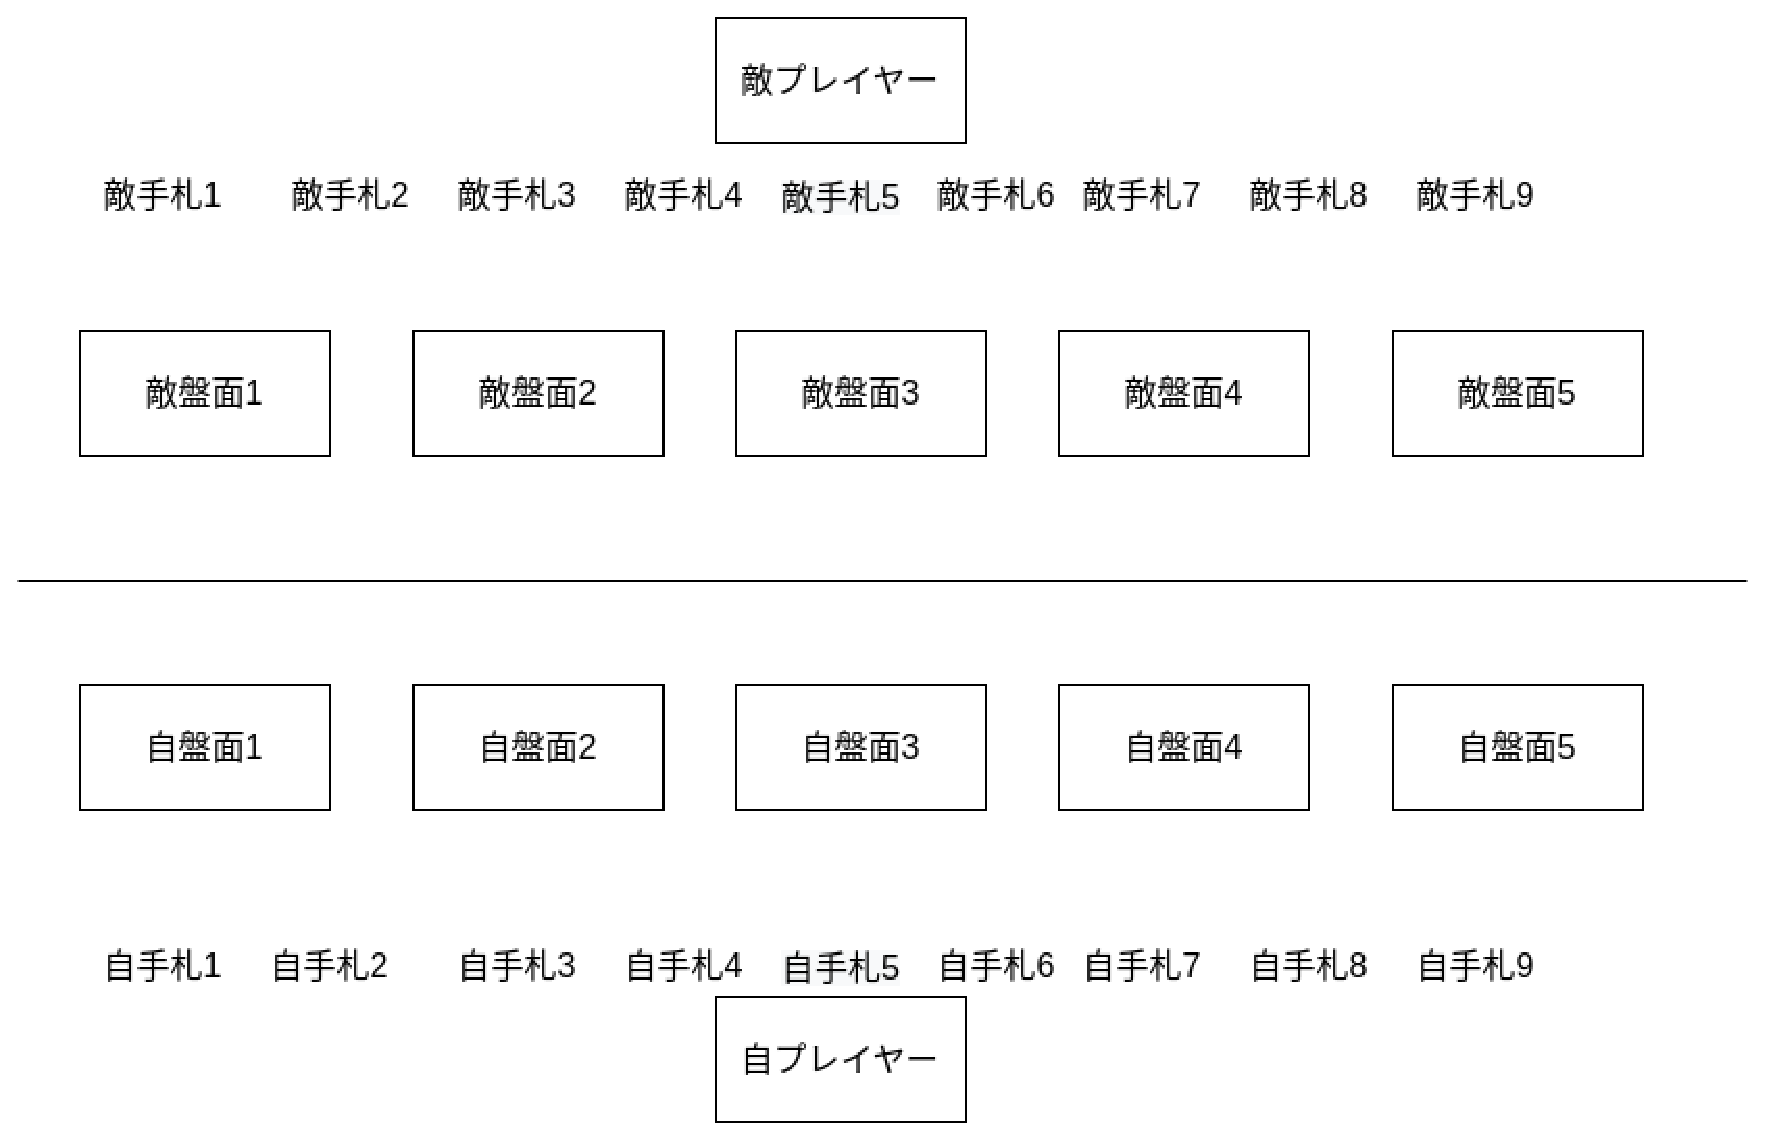
\includegraphics[width=150mm]{assets/Field.eps}
  \caption{定義した空間}
  \label{fig:Field}
\end{figure}

先週決めたように今回のルール設定では手札の最大枚数を 9, 盤面の最大枚数を 5 と決めている.
そのため,プレイヤーの行動は
\begin{quote}
  \begin{itemize}
   \item 自手札 1 - 9 を盤面に出す ・・・ 9 通り
   \item 自盤面 1 - 5 が敵盤面 1 - 5 を攻撃 ・・・ 5 * 5 = 25 通り
   \item ターンエンド ・・・ 1 通り
  \end{itemize}
 \end{quote}
の計 35 通りとなり, 行動空間の次元は 35 次元と定義した.


\subsection{状態空間の定義}
プレイヤーの観測できる状態として以下の計 43 個のパラメータを定義した.
\begin{quote}
  \begin{itemize}
   \item 自手札 1 - 9 の攻撃力と HP ・・・ 18 個
   \item 自盤面 1 - 5 の攻撃力と HP ・・・ 10 個
   \item 敵盤面 1 - 5 の攻撃力と HP ・・・ 10 個
   \item 自盤面 1 - 5 がターン中行動可能か ・・・ 5 個
  \end{itemize}
 \end{quote}

\subsection{報酬}
最適な報酬の与え方はまだ定まってはいないが,以下で述べる実験で採用した報酬設定は以下の通りである.なお,学習する側のプレイヤーの 1 行動を 1 ステップ,ゲーム開始から終了までを 1 エピソードとしている.

\begin{equation*}
  \mathrm{1 ステップ終了後}
  \quad reward \text{ = }
  \left\{
    \begin{aligned}
        1.0 \quad &(後攻プレイヤーのターン終了時先述の勝利条件で勝利していた場合) \\
        -1.0 \quad  &(後攻プレイヤーのターン終了時先述の勝利条件で敗北していた場合) \\
        -30.0 \quad & (ターンが回ってきたステップで即ターンエンドした場合) \\
        0.0 \quad &(otherwise)
    \end{aligned}
    \right.
\end{equation*}
\par
\begin{equation*}
  \mathrm{1 エピソード終了後}
  \quad reward \text{ = }
  \left\{
    \begin{aligned}
        10.0 \quad &(先述の勝利条件で勝利していた場合) \\
        -10.0 \quad  &(先述の勝利条件で敗北していた場合) \\
    \end{aligned}
    \right.
\end{equation*}

カードの枚数が同じだった場合にドローとしない, 即ターンエンドにペナルティをつける, 後攻プレイヤーの行動後に 0.0 以外の報酬を渡す用に設定した理由としては, 後述する実験においてこれら 3 つの処理を行わなかった際に学習が安定しなかったためである.環境から与えられる報酬が疎となるためと考えられる.

\subsection{実験設定}
作成した環境で学習できるか,また学習結果は妥当性のある結果となるか検証するために以下の設定で実験した.\par
学習するのは先攻プレイヤーであり,後攻プレイヤーは毎ターン 1 枚盤面にカードを出しその後は盤面にある行動可能なカードでランダムに対象を選択して攻撃する.
先攻,後攻プレイヤーのデッキを表 \ref{table:deck} に示す.

\begin{table}[h]
  \centering
  \caption{先攻, 後攻プレイヤーのデッキ\\
  ()内の数字は (攻撃力 , HP) を意味している.}
  \begin{tabular}{ll}
  \multicolumn{1}{c}{先攻} & \multicolumn{1}{c}{後攻} \\
  \hline
  ( 3 , 3 ) × 5          & ( 3 , 3 )  × 6         \\
  ( 2 , 3 ) × 5          & ( 1 , 5 ) × 3          \\
  ( 2 , 4 ) × 5          & ( 4 , 2 ) × 3          \\
                         & ( 3 , 2 ) × 3         \\
  \hline
  \label{table:deck}
  \end{tabular}
\end{table}

また実験では Deep-Q-Network であるステップ回学習を行い, 10000 エピソード検証し勝率を求める.
この操作を 10000, 50000, 100000, 150000, 200000 ステップと変更して行い勝率を比較した.

図 \ref{fig:model} , 表 \ref{table:param} に実験で使用したモデルとモデルのパラメータ設定を示す.

\begin{table}[h]
  \centering
  \caption{DQNのパラメータ\cite{パラメータ}}
  \label{table:param}
  \begin{tabular}{|c||c|}
  \hline
  方策                 & ε-greedy \\ \hline
  ε                      & 0.1      \\ \hline
  全結合層の活性化関数             & ReLU     \\ \hline
  全結合層の次元                & 16       \\ \hline
  最適化アルゴリズム              & Adam     \\ \hline
  学習率                    & 1e-3     \\ \hline
  Experience Replayのメモリ量 & 1000000  \\ \hline
  \end{tabular}
  \end{table}

  \begin{figure}[htbp]
    \centering
    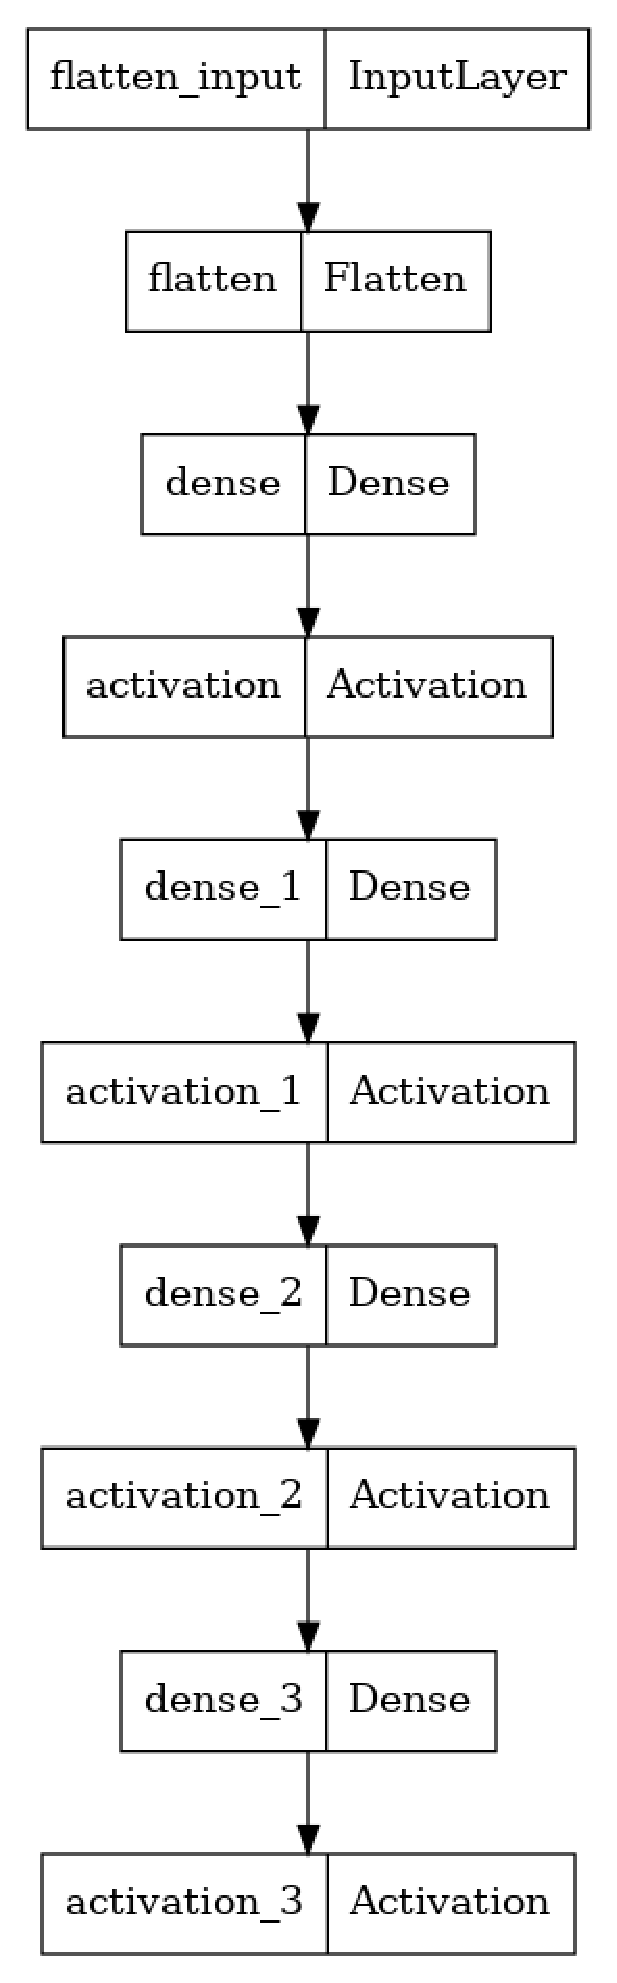
\includegraphics[width=60mm]{assets/model.eps}
    \caption{実験で用いたモデル}
    \label{fig:model}
  \end{figure}
\subsection{実験結果}
勝率は 10000 エピソードの検証を 5 回行いその平均値を用いた.
結果を表 \ref{table:result} に示す.

  
\begin{table}[h]
  \centering
  \caption{各ステップ数における勝率}
  \label{table:result}
  \scalebox{1.5}[1.5]{
    \begin{tabular}{|c|c|}
      \hline
      ステップ数  & 勝率      \\ \hline
      10000  & 0.57336 \\ \hline
      50000  & 0.63074 \\ \hline
      100000 & 0.62650 \\ \hline
      150000 & 0.71484 \\ \hline
      200000 & 0.70110 \\ \hline
      \end{tabular}
  }
  \end{table}

  また,各ステップ数の実験時のエピソードごとのreward, stepの推移を図 3 - 7 に示す.

  \begin{figure}[htbp]
    \centering
    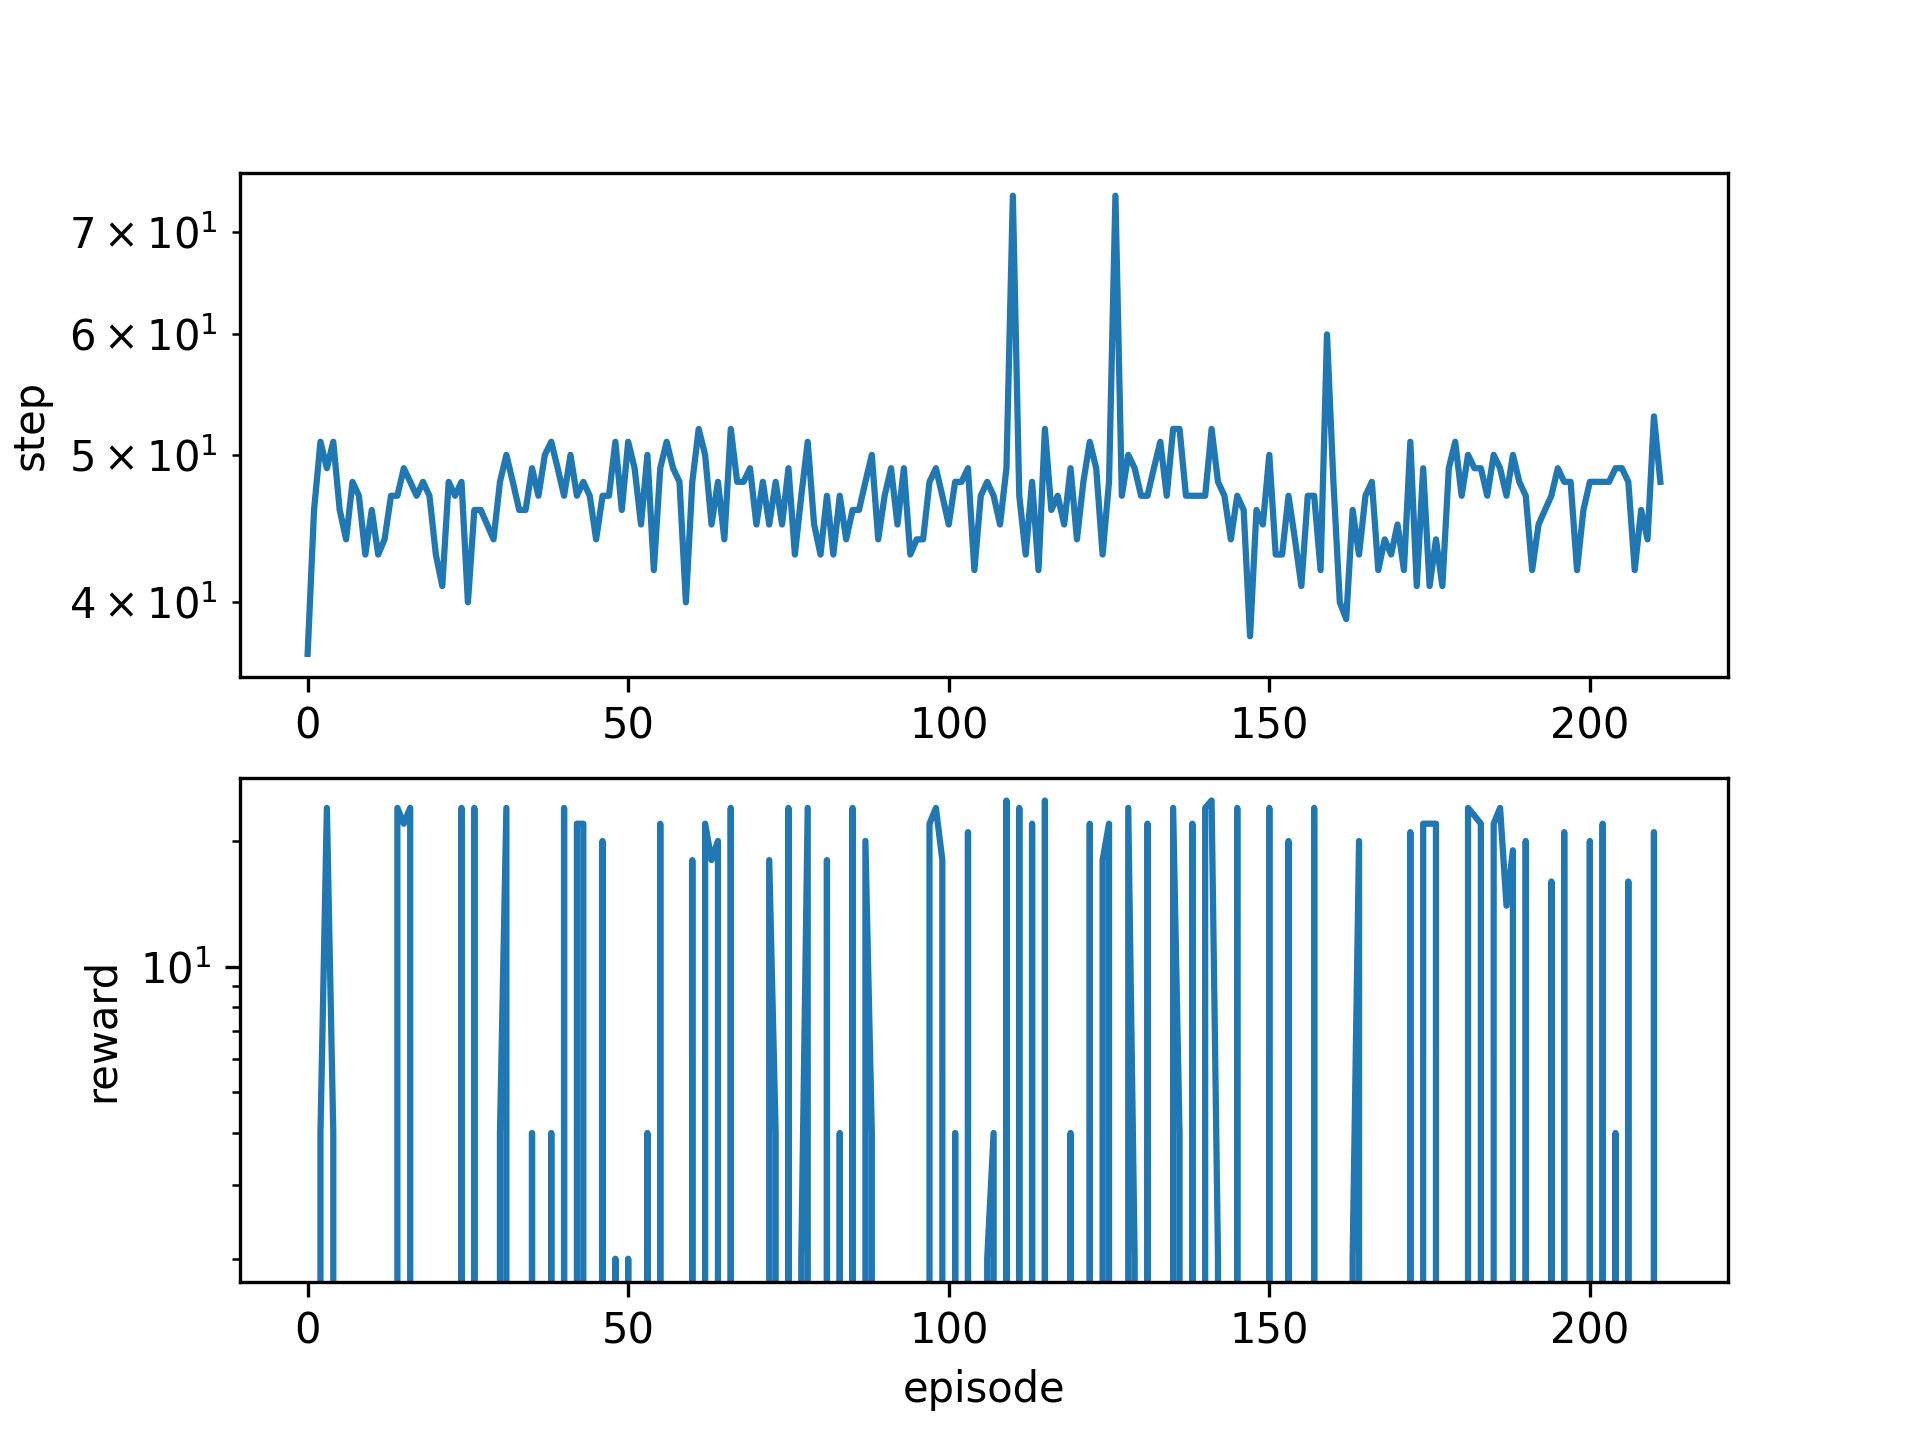
\includegraphics[width=120mm]{assets/10000.eps}
    \caption{ステップ数10000の際の推移}
    \label{fig:10000}
  \end{figure}
  \begin{figure}[htbp]
    \centering
    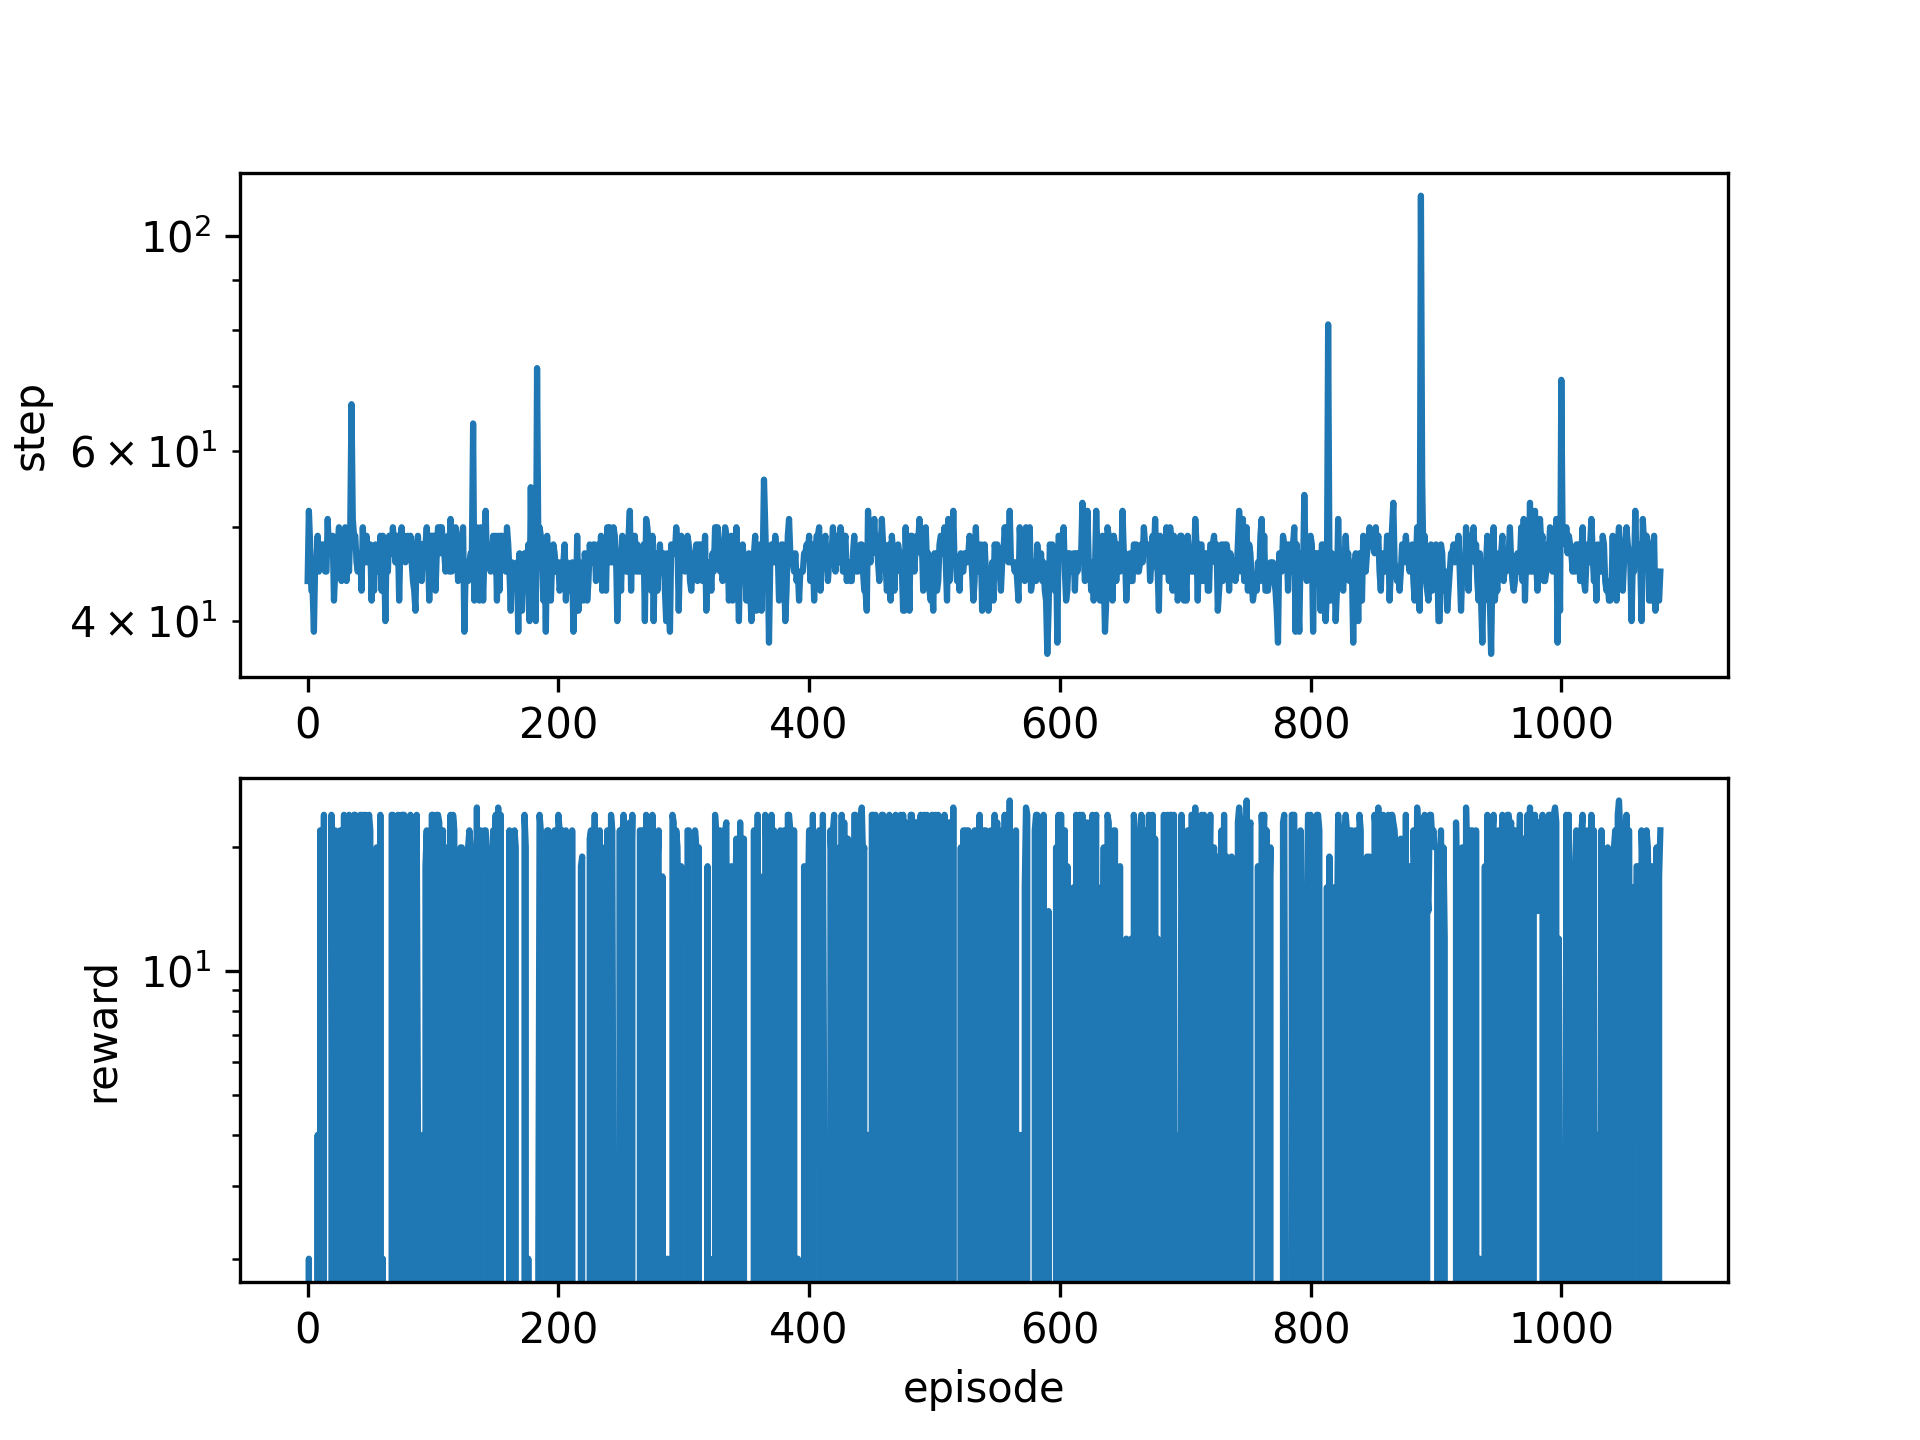
\includegraphics[width=120mm]{assets/50000.eps}
    \caption{ステップ数50000の際の推移}
    \label{fig:50000}
  \end{figure}
  \begin{figure}[htbp]
    \centering
    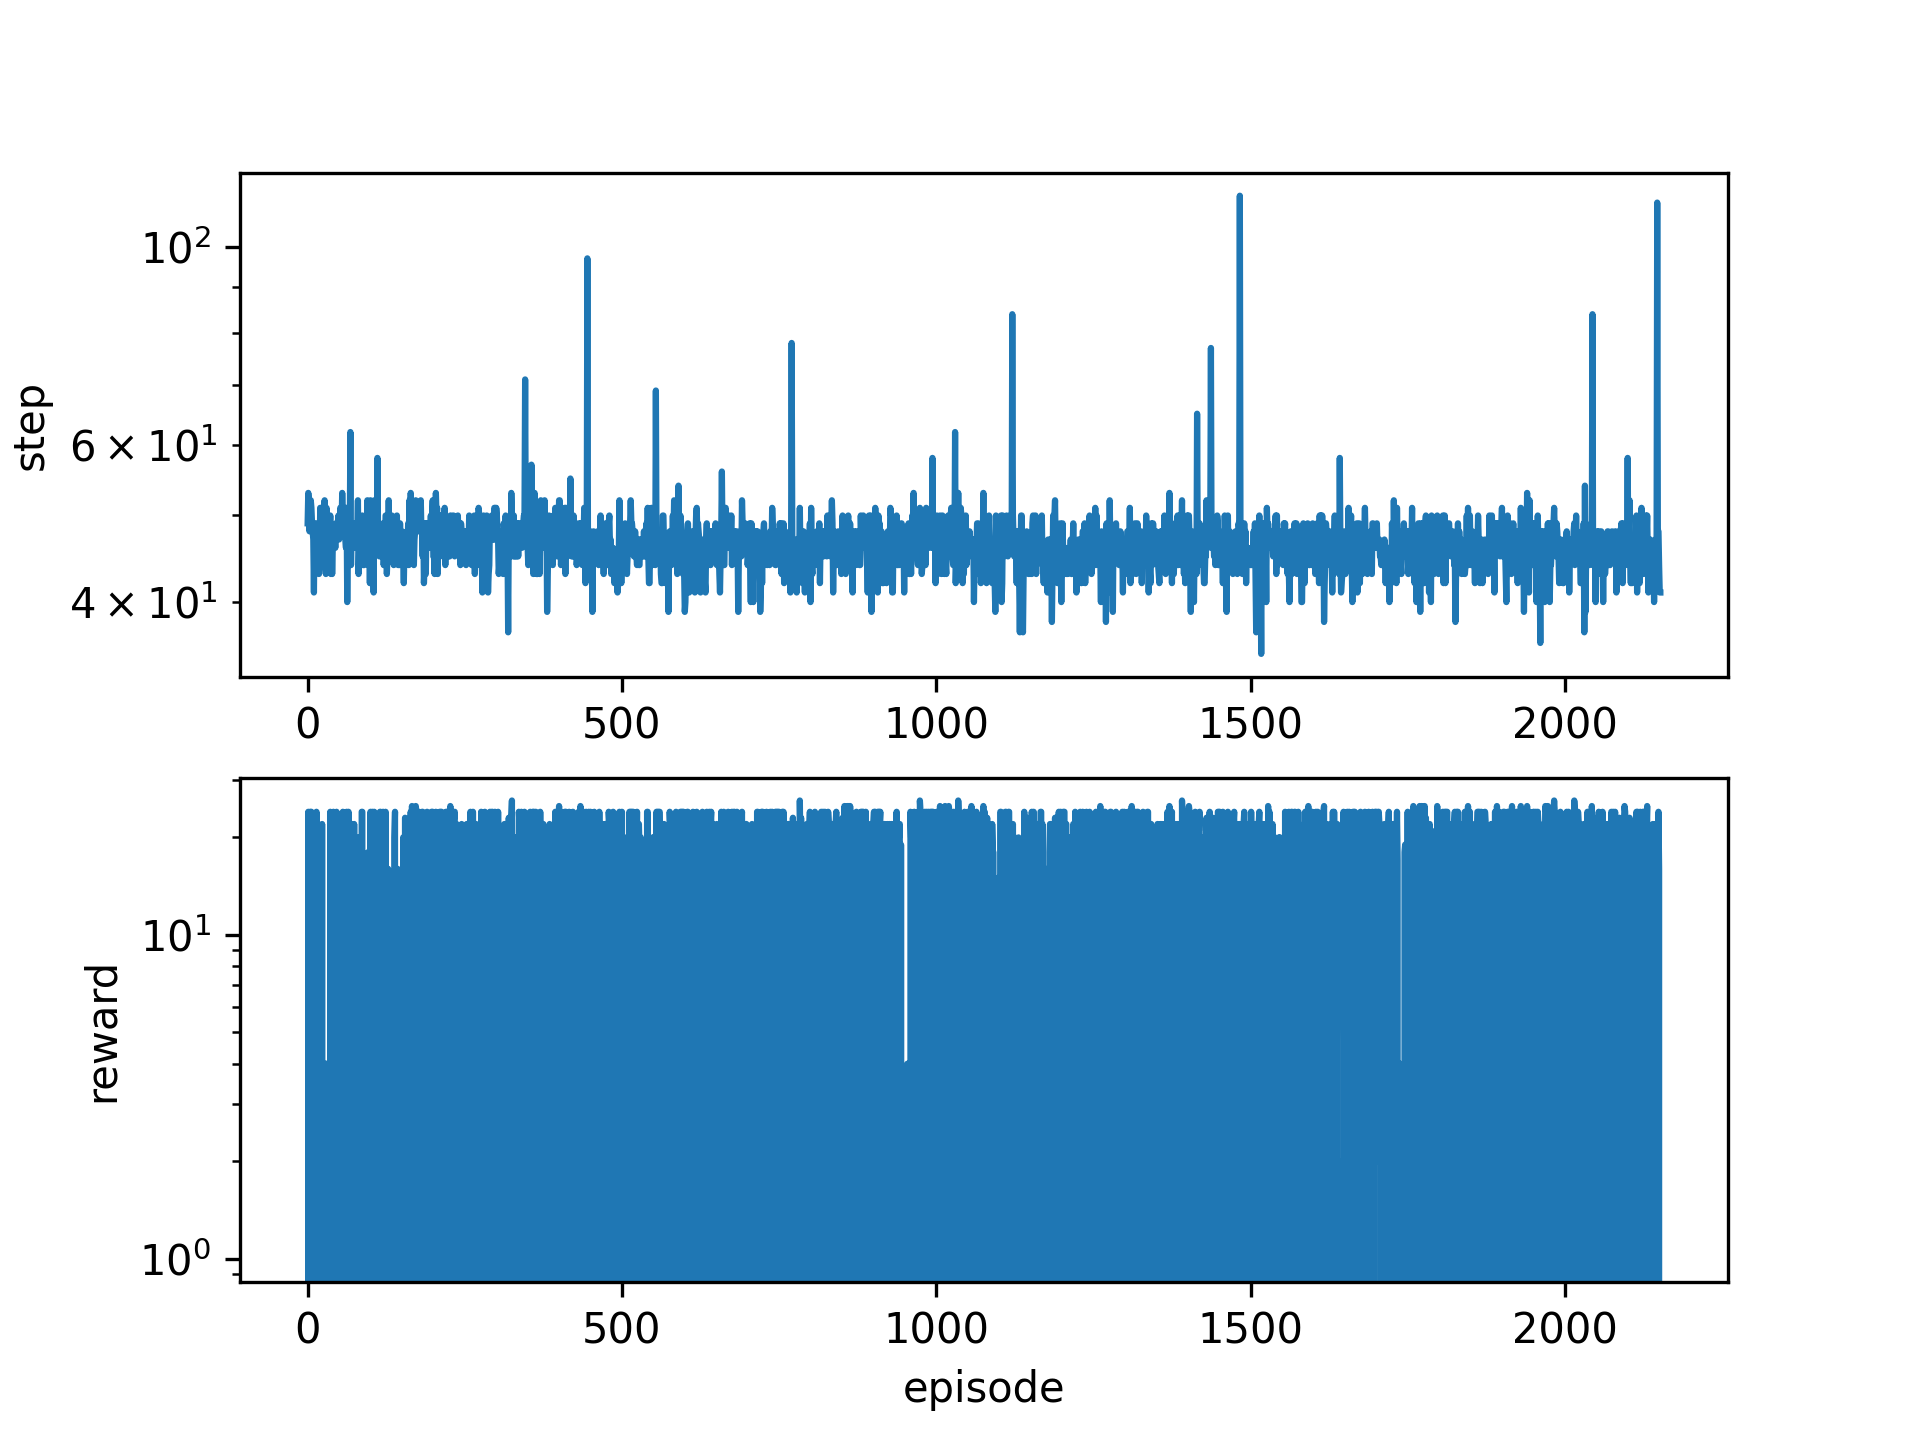
\includegraphics[width=120mm]{assets/100000.eps}
    \caption{ステップ数100000の際の推移}
    \label{fig:100000}
  \end{figure}
  \begin{figure}[htbp]
    \centering
    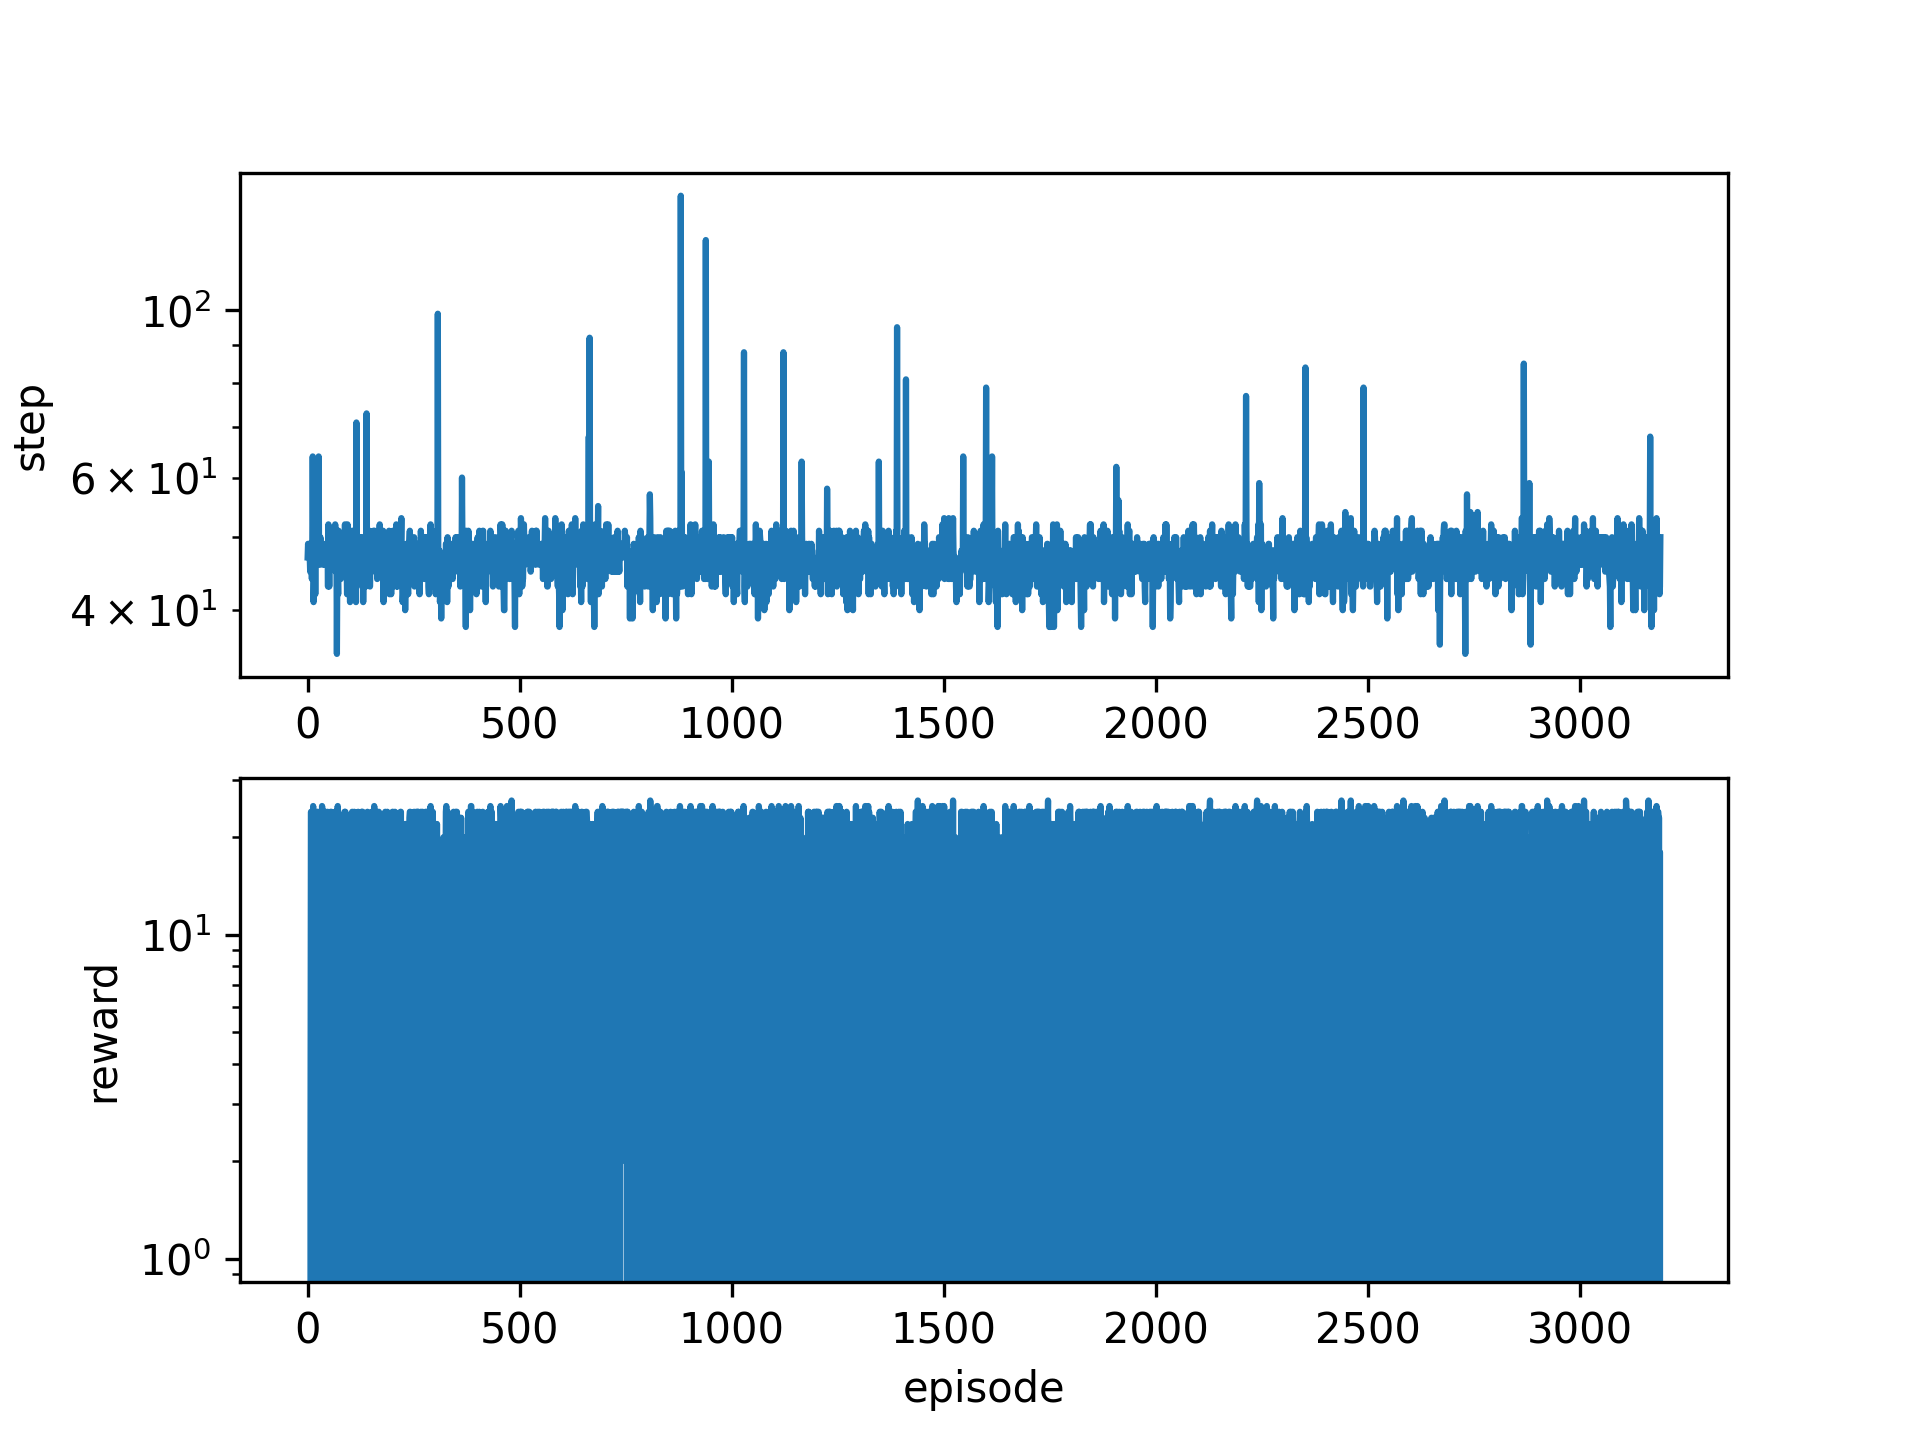
\includegraphics[width=120mm]{assets/150000.eps}
    \caption{ステップ数150000の際の推移}
    \label{fig:150000}
  \end{figure}
  \begin{figure}[htbp]
    \centering
    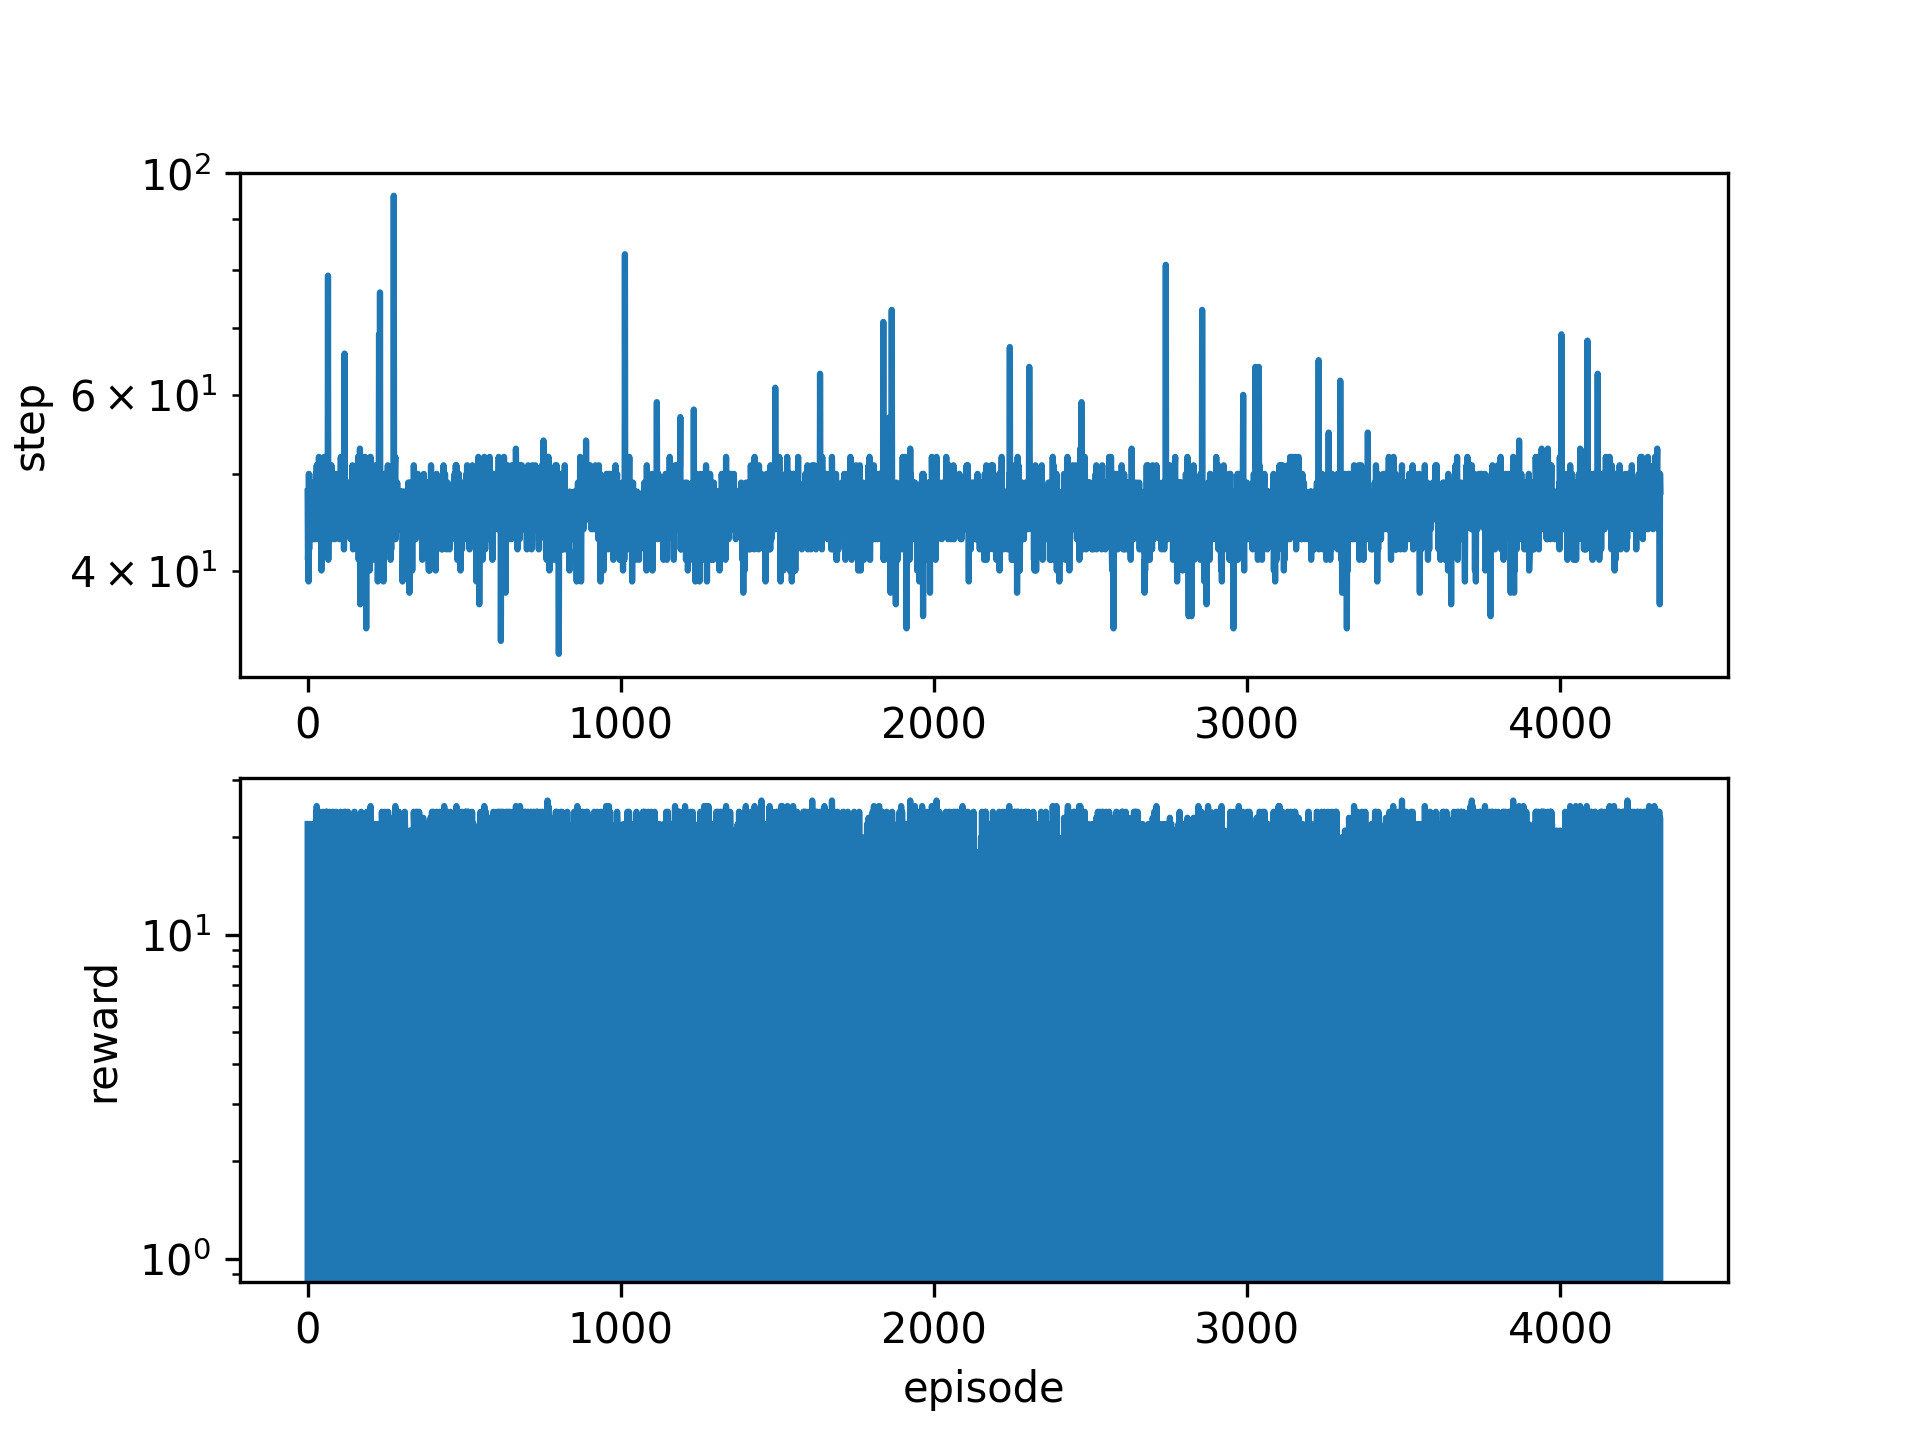
\includegraphics[width=120mm]{assets/200000.eps}
    \caption{ステップ数200000の際の推移}
    \label{fig:200000}
  \end{figure}


\subsection{考察,検討}
多少の誤差はあれどステップが増えれば勝率は上がっているといえる.ただ,デッキのシャッフルや相手の行動でランダム要素が含まれているとはいえ勝率 7 割という数値が妥当性があるかは検討の余地がある.
学習率のパラメータを調整する必要があるのか,報酬の与え方に問題があるのか,どちらにせよモデルと環境側それぞれについて検討していきたい. また keras と Optuna を用いてパラメータの調整を行っている参考資料も見つけたので Optuna といったフレームワークも試してみたい\cite{Optuna}. \par
また, 本資料を書いている途中に気づいたが行動次元数が 35 であるにもかかわらずモデルの全結合層の次元が 16 であったり, デッキにおいてカードのパラメータは先週の実験の数値を使いまわしており HP が低く盤面に残りづらいという問題があるため修正し再実験する必要があると言える.

\subsection{今後やること}

\begin{quote}
  \begin{itemize}
    \item 再実験
    \par
    今回作成した環境で上手く学習できればやっと環境構築から開放されるので早めに確認・修正する.
   \item モンテカルロ法の実装
   \par
   環境の改良に時間がかかってしまったため先延ばしになってしまった.kerasの Agent クラスをオーバーライドしても上手く行かなさそうなので 1 から作ってみる.また,keras-rl を用いると DDQN や DDPG といった深層強化学習手法も簡単に試せそうであったため必要があれば試してみたい\cite{Document}.

   \item 自動バランス調整の方法検討
   知識不足で見当がつかないので調べる.
   
  \end{itemize}
 \end{quote}

%index.bibはtexファイルと同階層に置く
%ちゃんと\citeしないと表示されない(1敗)
\bibliography{index.bib}
\bibliographystyle{junsrt}

\end{document}